\documentclass[letterpaper,12pt]{article}
\usepackage{tabularx} % extra features for tabular environment
\usepackage{amsmath}  % improve math presentation
\usepackage{float}
\usepackage{pdfpages}

\usepackage{graphicx} % takes care of graphic including machinery
\graphicspath{ {./figures/} }
\usepackage[margin=1in,letterpaper]{geometry} % decreases margins
\usepackage{cite} % takes care of citations
\usepackage[final]{hyperref} % adds hyper links inside the generated pdf file
\hypersetup{
	colorlinks=true,       % false: boxed links; true: colored links
	linkcolor=blue,        % color of internal links
	citecolor=blue,        % color of links to bibliography
	filecolor=magenta,     % color of file links
	urlcolor =blue         
}

%



\begin{document}

\title{Experiment 6 Preliminary Work \protect\\ Operational Amplifiers - II}
\author{Ahmet Akman 2442366 \protect\\}
\date{\today}
\maketitle
\newpage
\tableofcontents
\newpage
%\begin{abstract}
%abstract
%\end{abstract}

\section{Introduction} 
In preliminary work of the Experiment 6 , the steps for the pre-experiment are conducted and presented.
\section{Step 1}
For this step circuit given in Figure 1 is taken as the reference.
\begin{figure}[H]
	\centering
   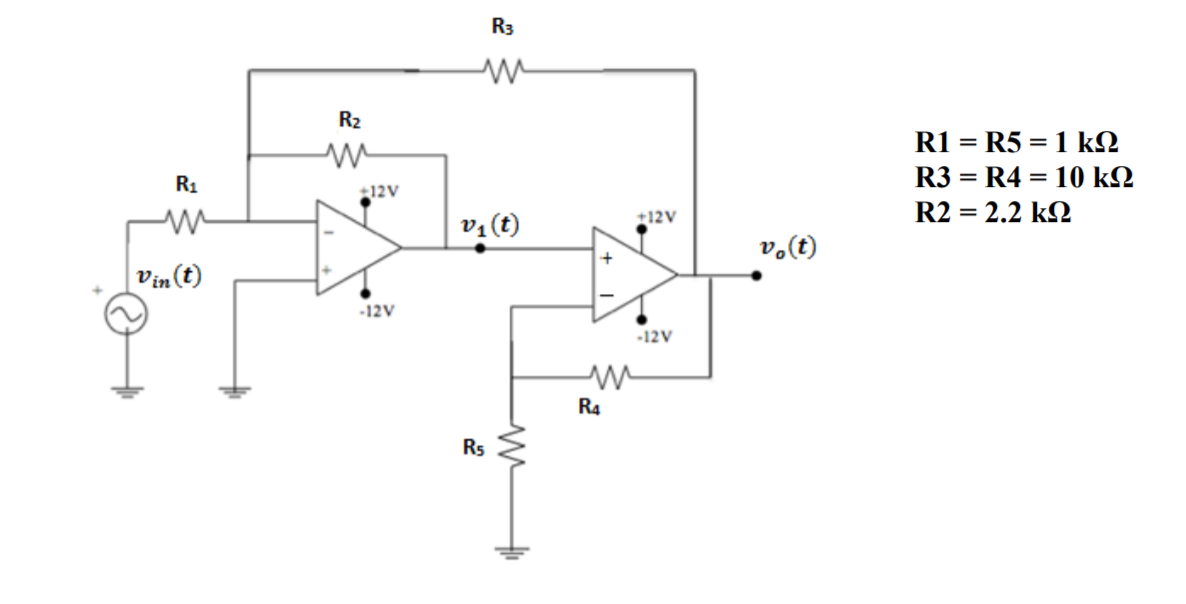
\includegraphics[width=0.8\textwidth]{circuit_1.png}
   \caption{Circuit schematic for the step 1}
\end{figure} 

\subsection{a)}
The expression relating \(V_o(t)\) to \(V_{in}\) is obtained via hand calculations which is given in Figure 2.

\begin{figure}[H]
	\centering
   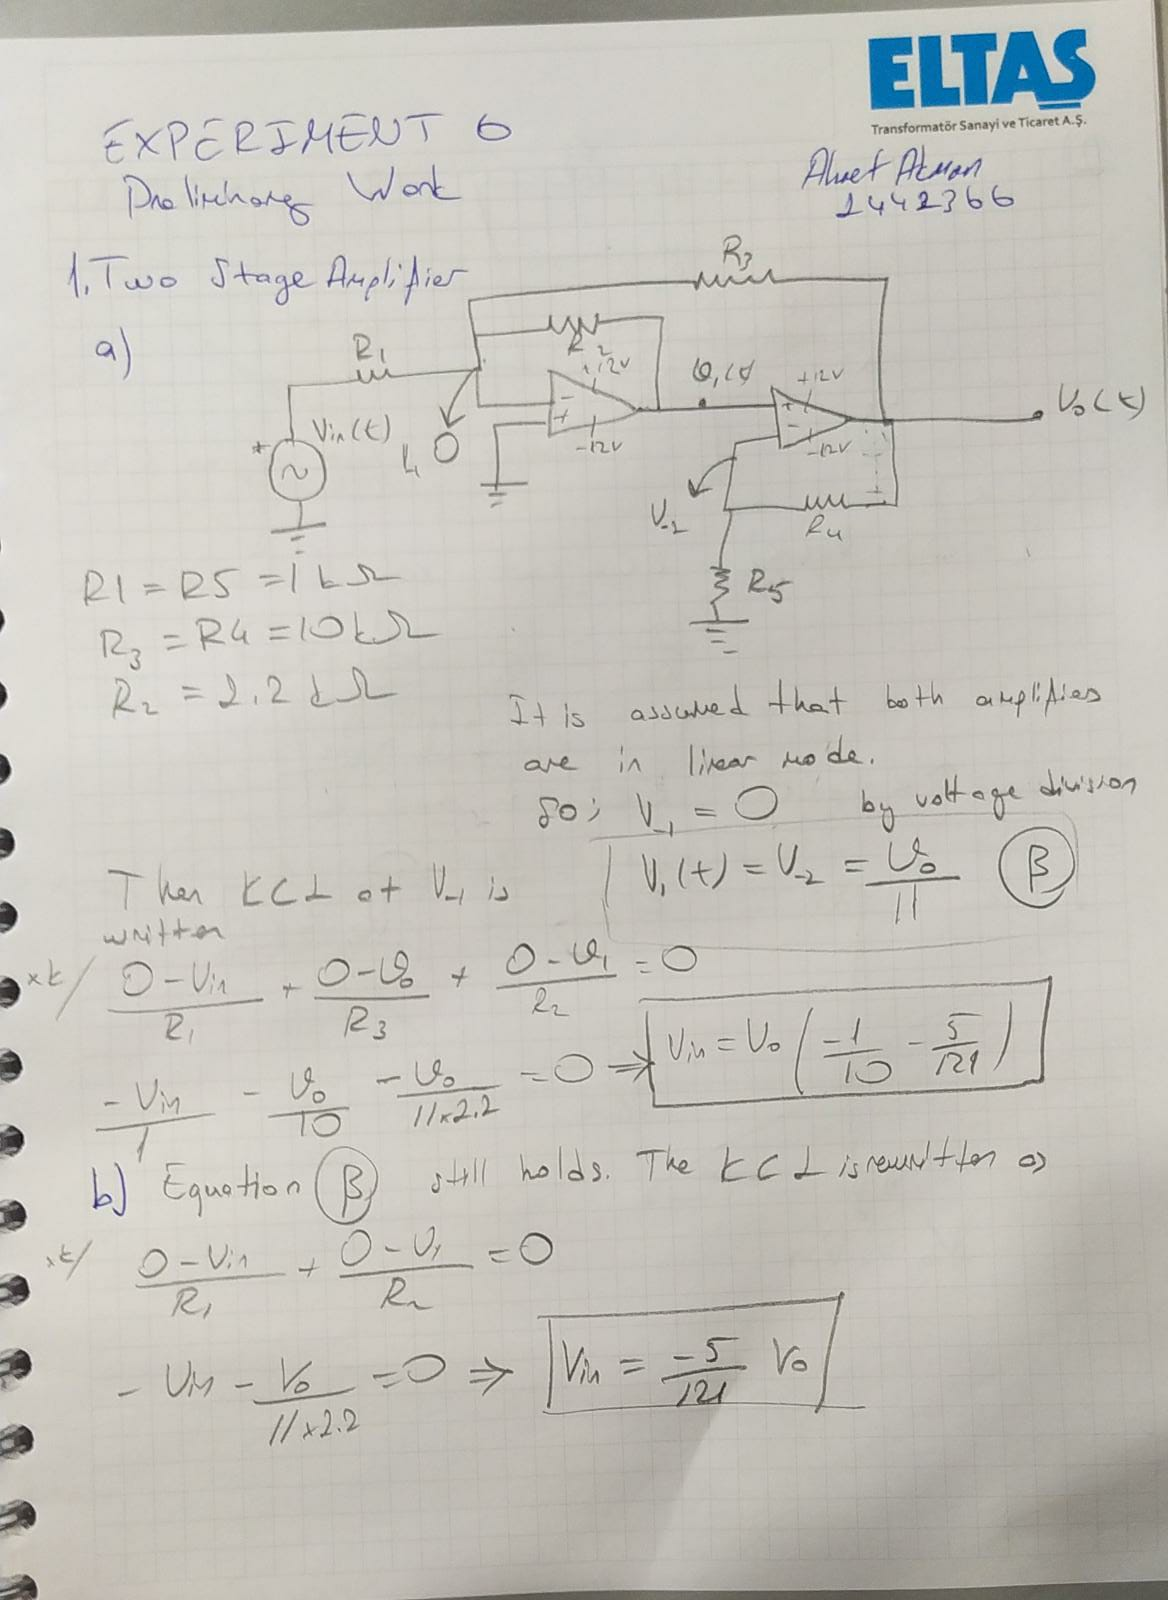
\includegraphics[width=0.6\textwidth]{1_hand.jpeg}
   \caption{Hand calculations for the expression relating \(V_o(t)\) to \(V_{in}\)}
\end{figure} 
\(V_o(t) vs V_{in}\) is sketched in the Figure 3 according to the calculations in Figure 2.
\begin{figure}[H]
	\centering
   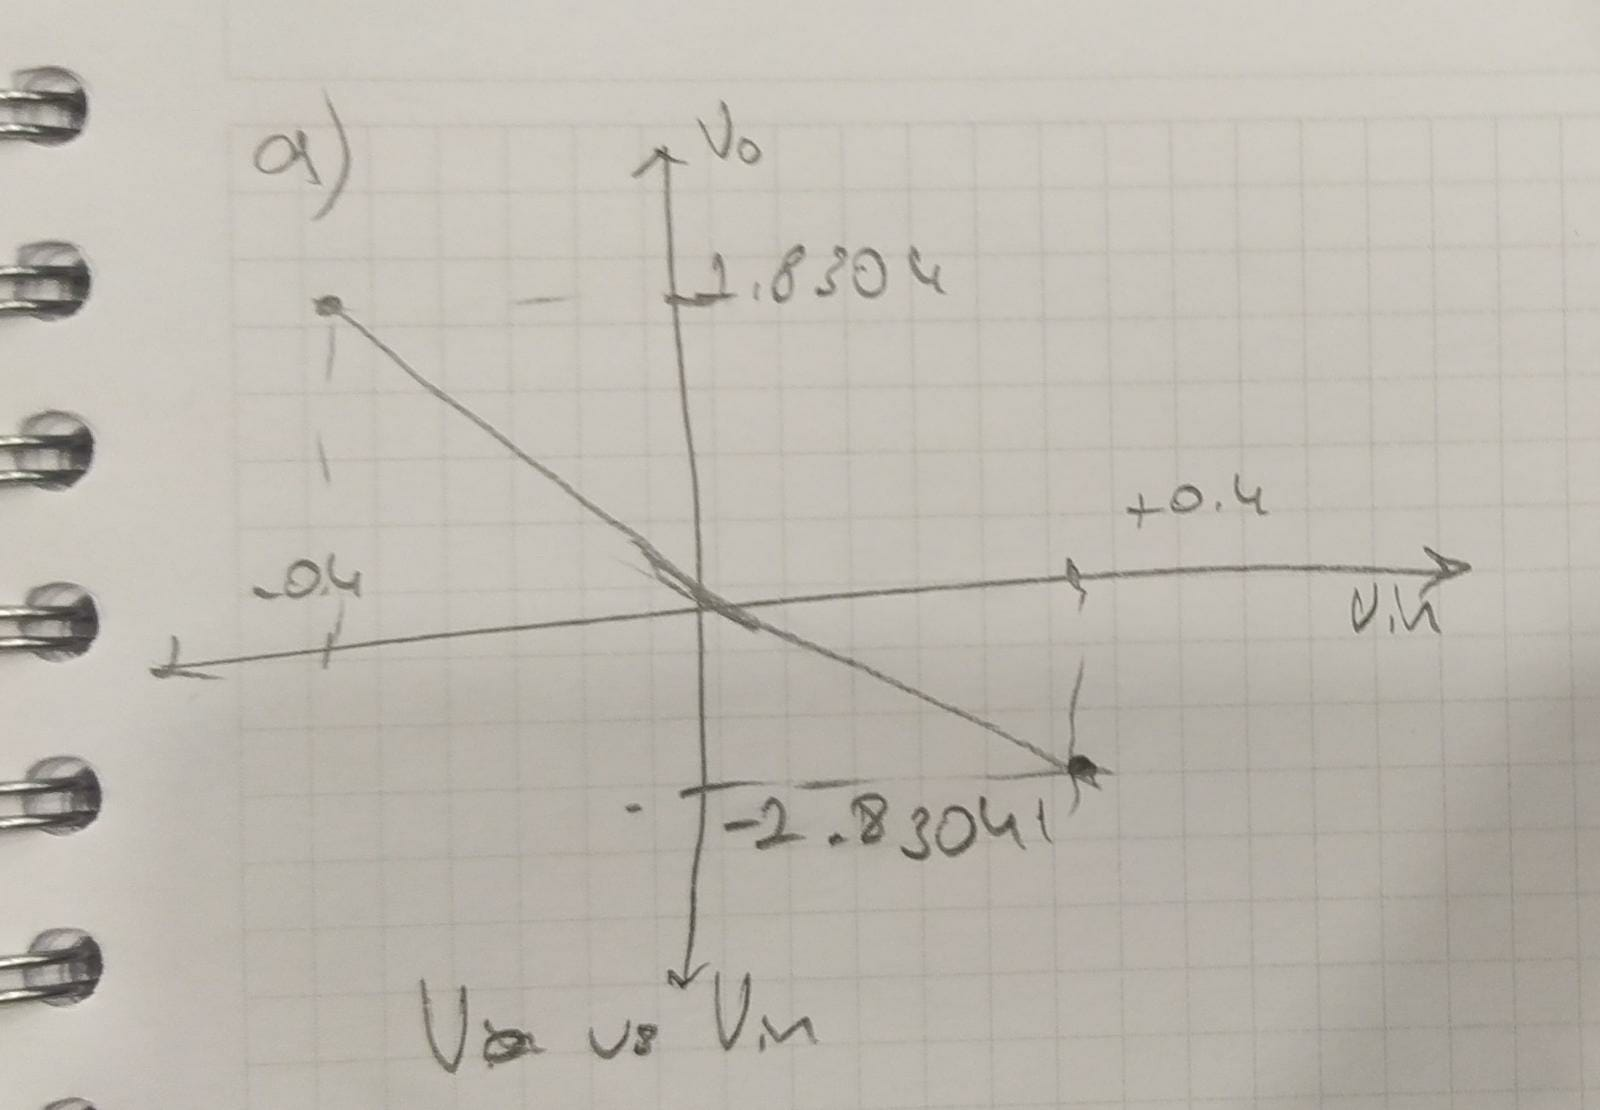
\includegraphics[width=0.6\textwidth]{1_a_sketch.jpeg}
   \caption{\(V_o(t) vs V_{in}\) sketch}
\end{figure} 
\subsection{b)}

The expression relating \(V_o(t)\) to \(V_{in}\) without R3 is obtained via hand calculations which is given in Figure 2.
\(V_o(t) vs V_{in}\) is sketched in the Figure 4 according to the calculations in Figure 2.
\begin{figure}[H]
	\centering
   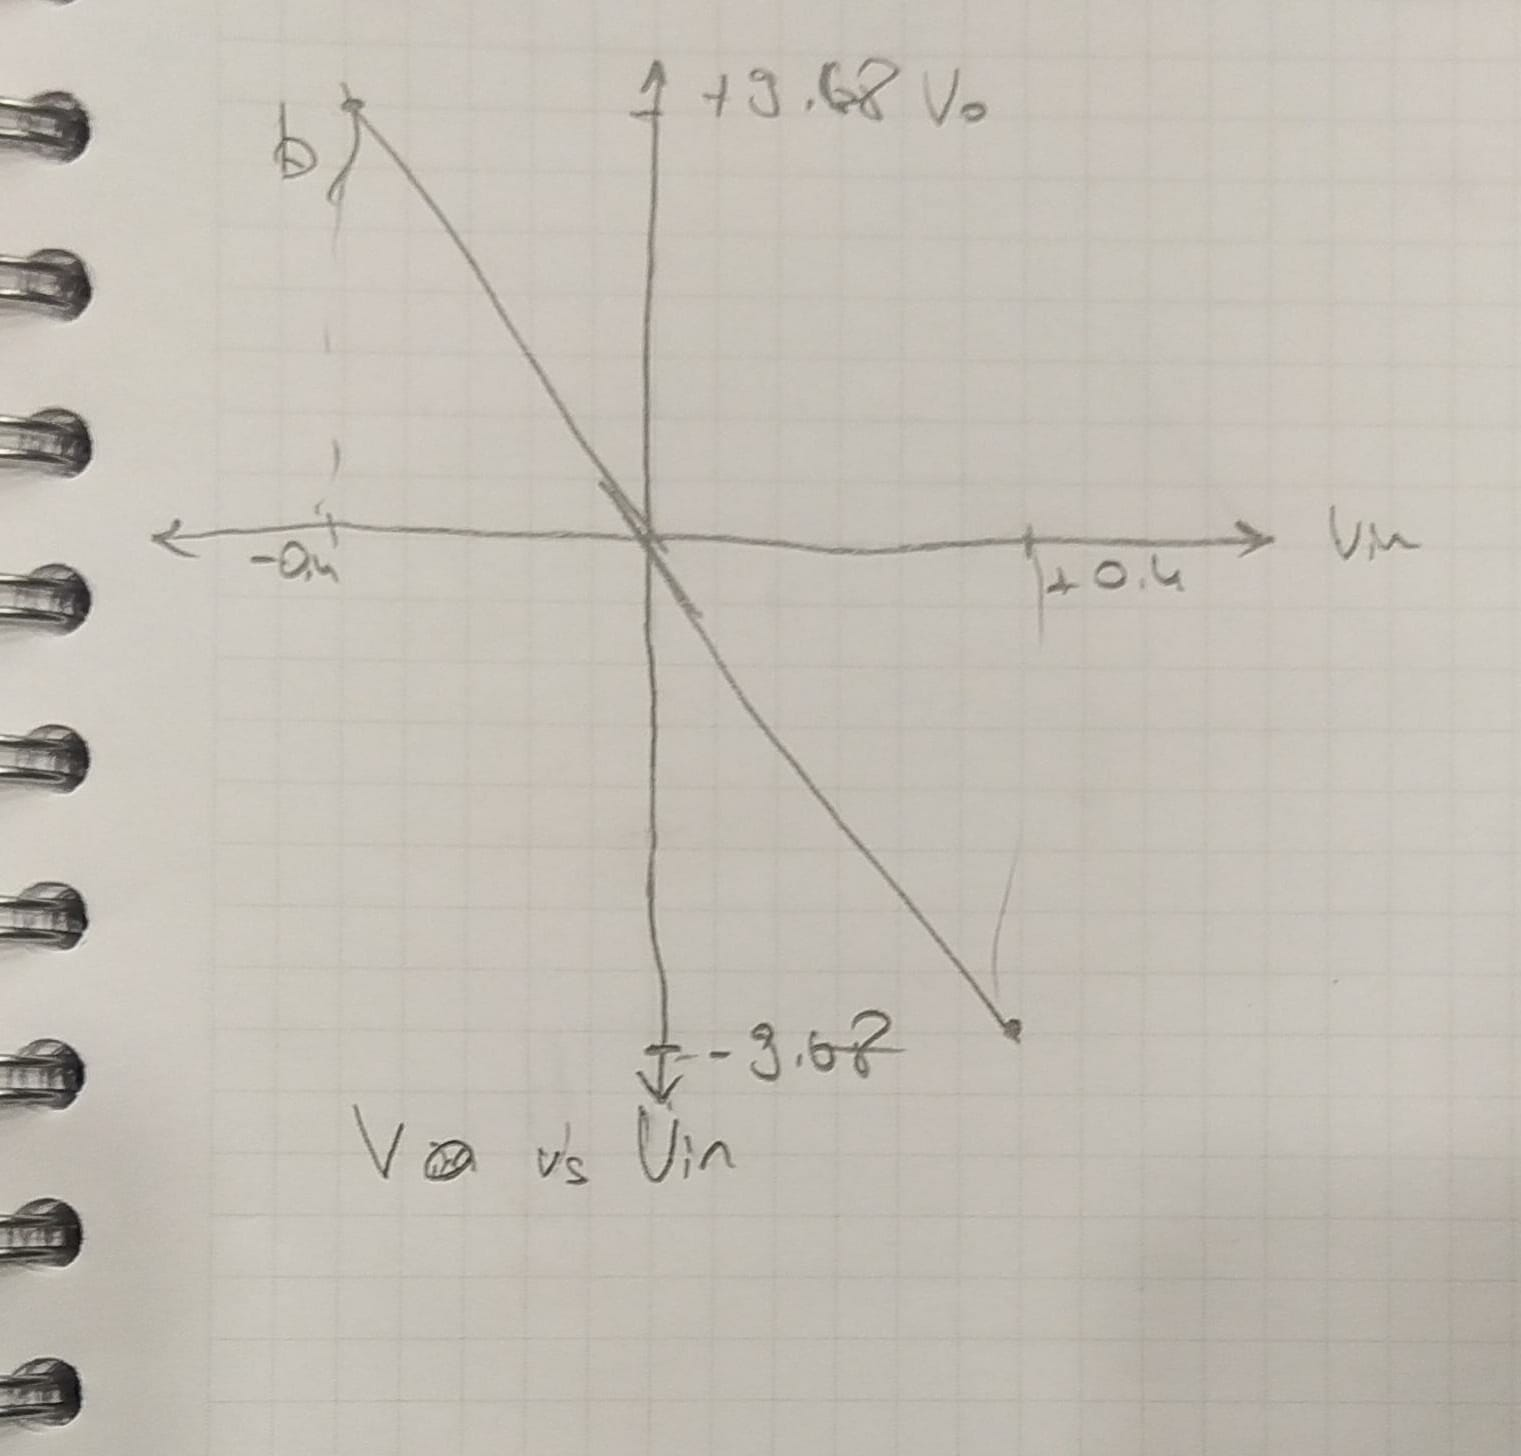
\includegraphics[width=0.6\textwidth]{2_b_sketch.jpeg}
   \caption{\(V_o(t) vs V_{in}\) sketch}
\end{figure} 

\section{Step 2}

For this step circuit given in Figure 5 is taken as the reference.
\begin{figure}[H]
	\centering
   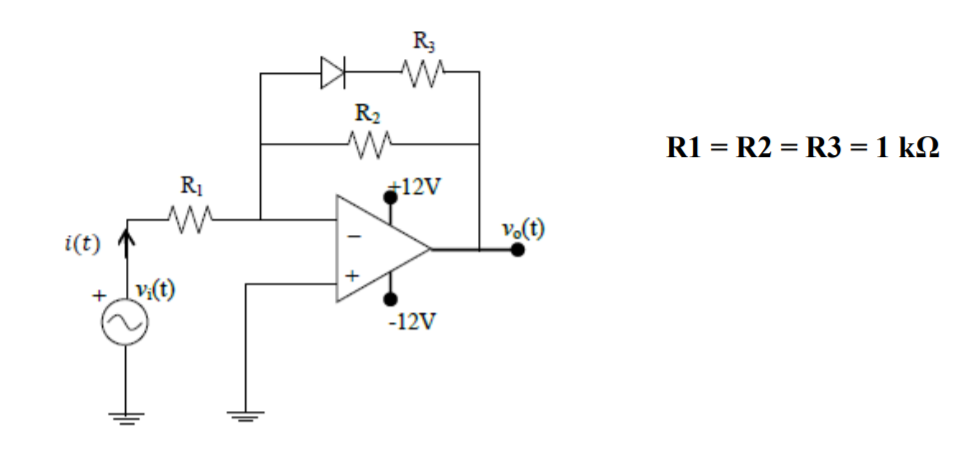
\includegraphics[width=0.6\textwidth]{circuit_2.png}
   \caption{Circuit for Step 2}
\end{figure} 

Then \(V_o vs V{in}\) is plotted given in Figure 6 with its calculations.
\begin{figure}[H]
	\centering
   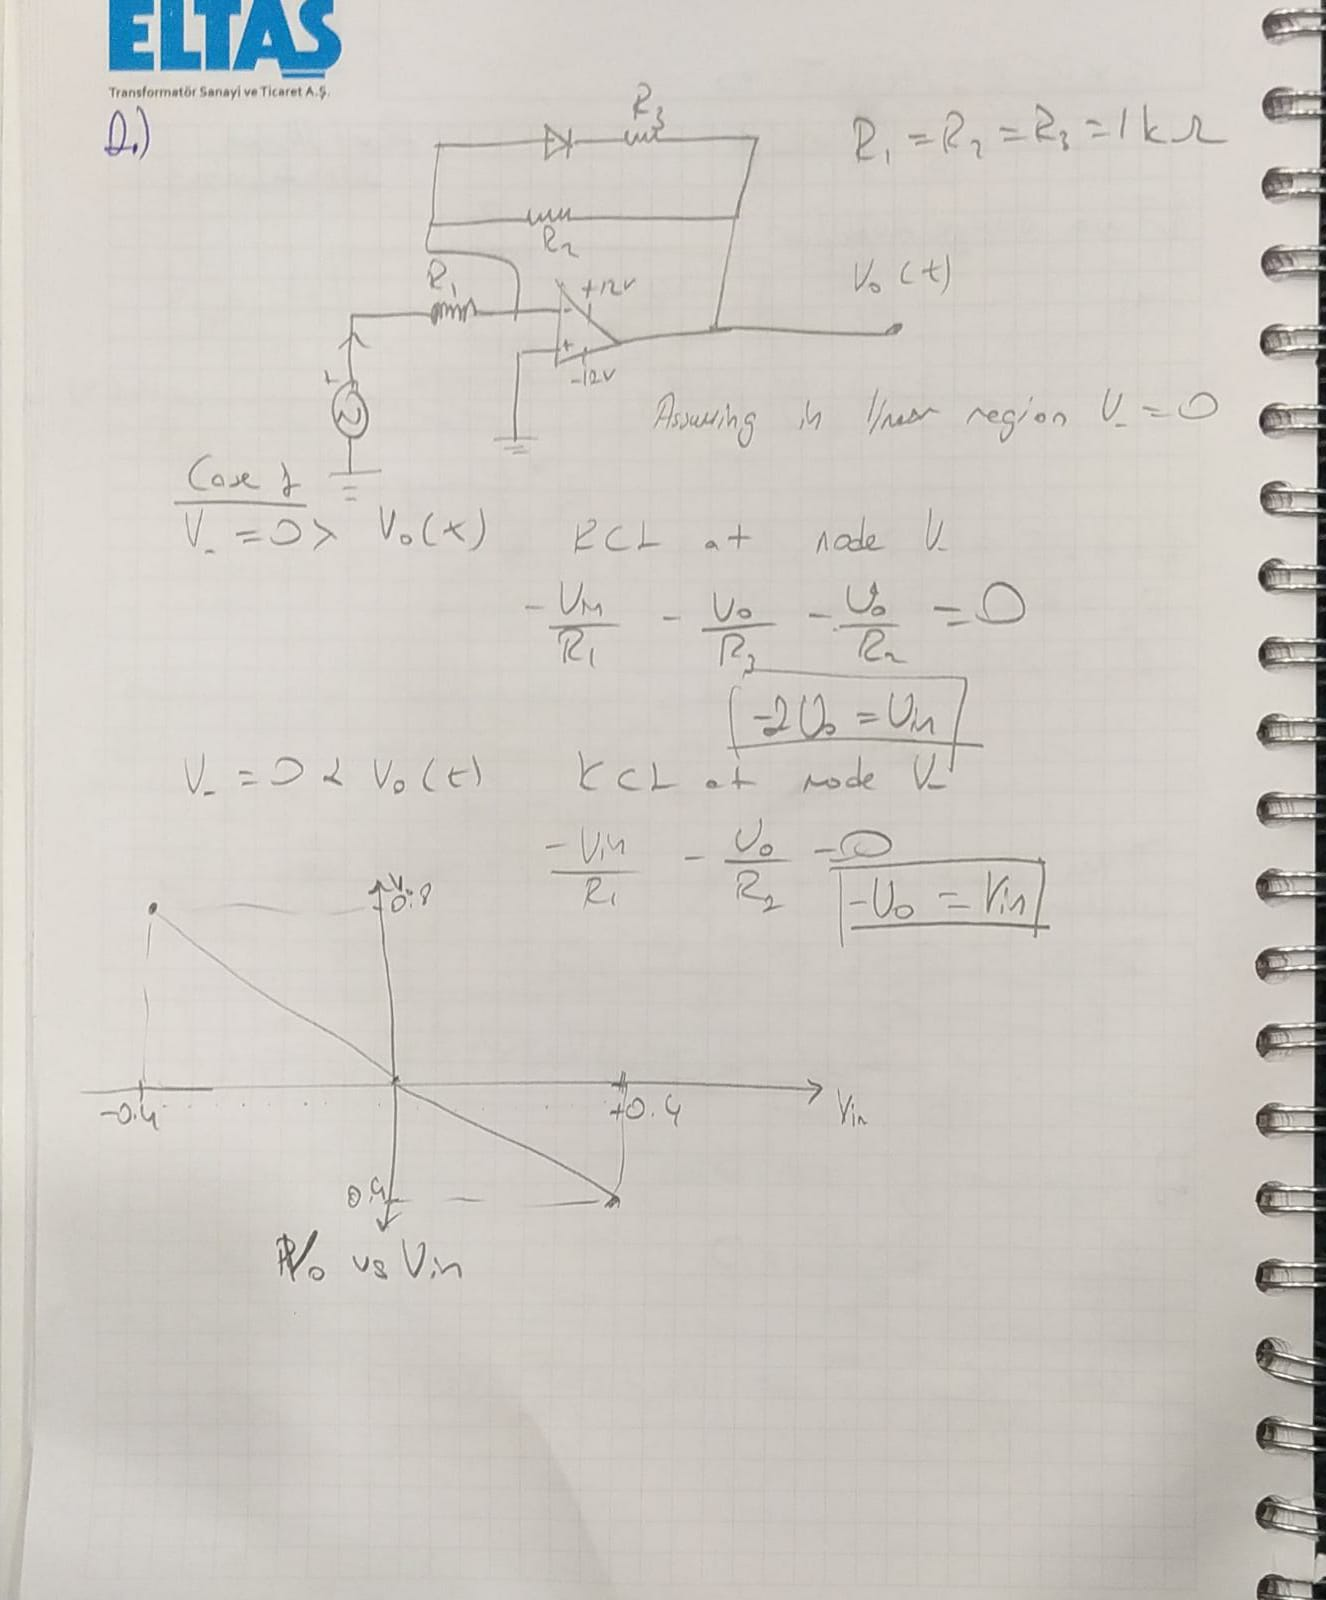
\includegraphics[width=0.6\textwidth]{2_hand.jpeg}
   \caption{\(V_o(t) vs V_{in}\) sketch}
\end{figure} 
In order to measure this characteristic using a DSO, the voltage difference between \(V_-\) and \(V_0\) should be increased so  that non-ideal diode (e.g. 1N007) react this difference properly. This can be done by increasing the \(V_{in}\) and/or decreasing the \(R_1\) 
\section{Step 3}
\subsection{a) Darkness Sensor}
The circuit given in Figure 7 is taken as the reference.
\begin{figure}[H]
	\centering
   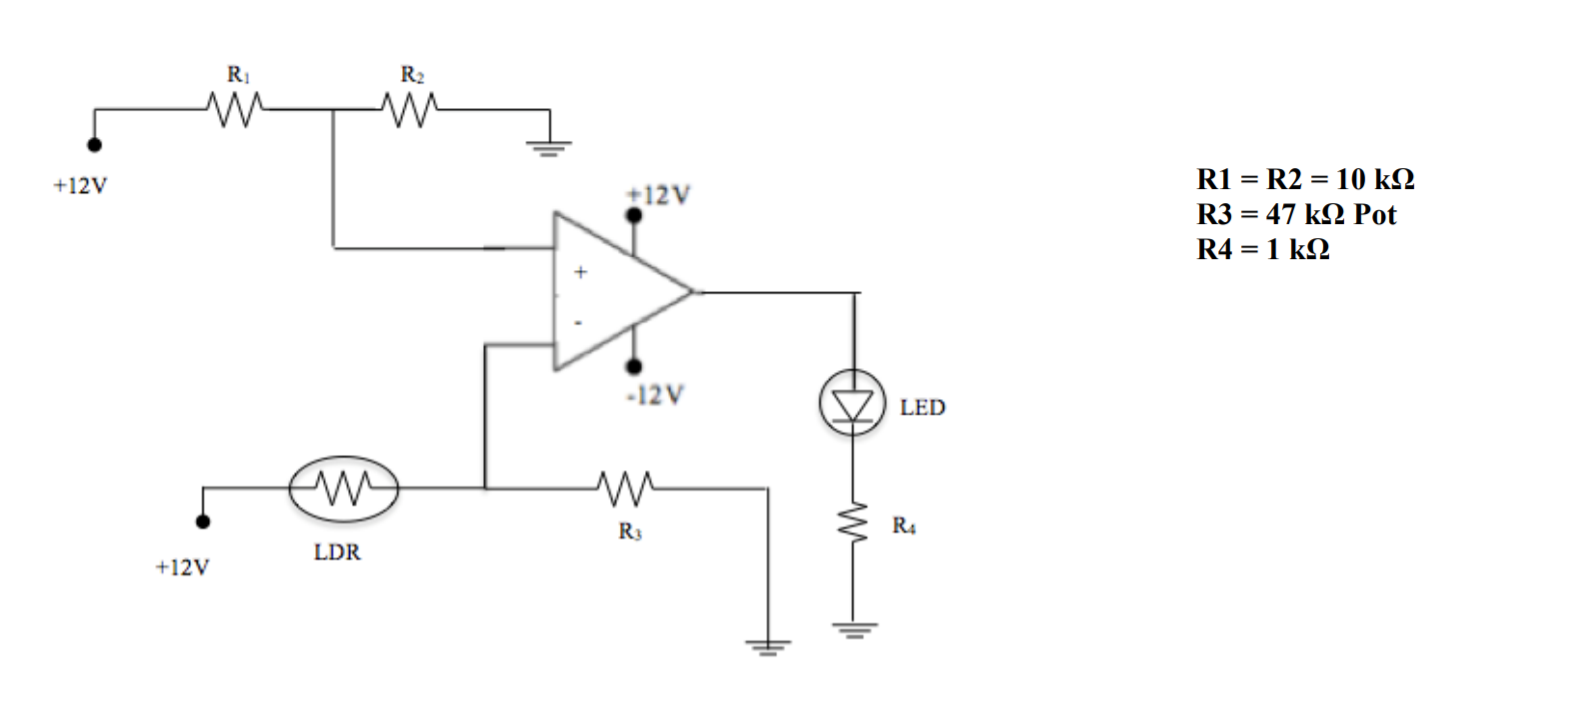
\includegraphics[width=0.8\textwidth]{darkness.png}
   \caption{Darkness sensor circuit for the Step 3}
\end{figure} 
The relation that express \(V_o(t) vs R_{LDR}\) can be derived using voltage divider equations as follows.
\[V_+ = 6 Volts
\]\[
V_- = 12\frac{R_3}{R_3+R_{LDR}}
\]
so;
\[ 
if (6-12\frac{R_3}{R_3+R_{LDR}} > 0, V_o = +12V)
\]\[ 
if (6-12\frac{R_3}{R_3+R_{LDR}} < 0, V_o = -12V)
\]
\subsection{b) Lightness Sensor}
The lightness sensor can be designed via swapping the inverting and non-inverting terminals of Op-Amp  in the circuit given in Figure 6. So the resulting circuit is given in the Figure 7.
\begin{figure}[H]
	\centering
   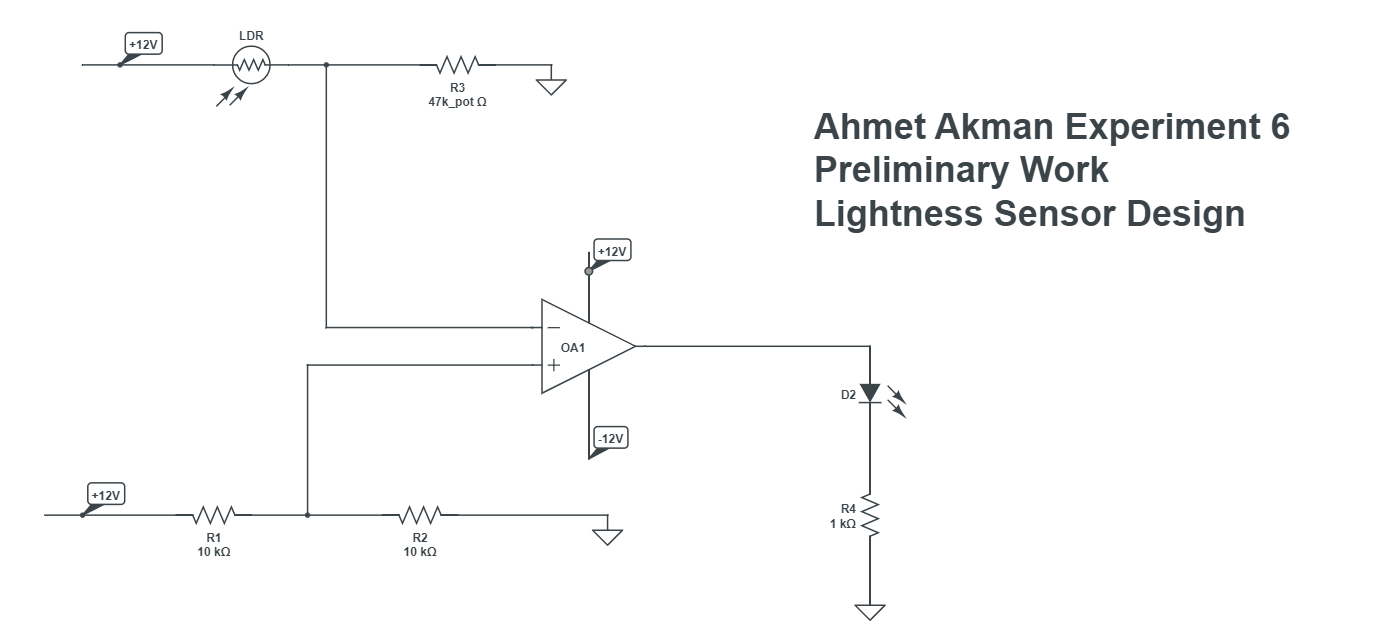
\includegraphics[width=1\textwidth]{lightness.png}
   \caption{Lightness sensor circuit for the Step 3}
\end{figure} 

\section{Step 4}
The circuit in the Figure 1 is constructed in LTSpice environment, given in Figure 8.
\begin{figure}[H]
	\centering
   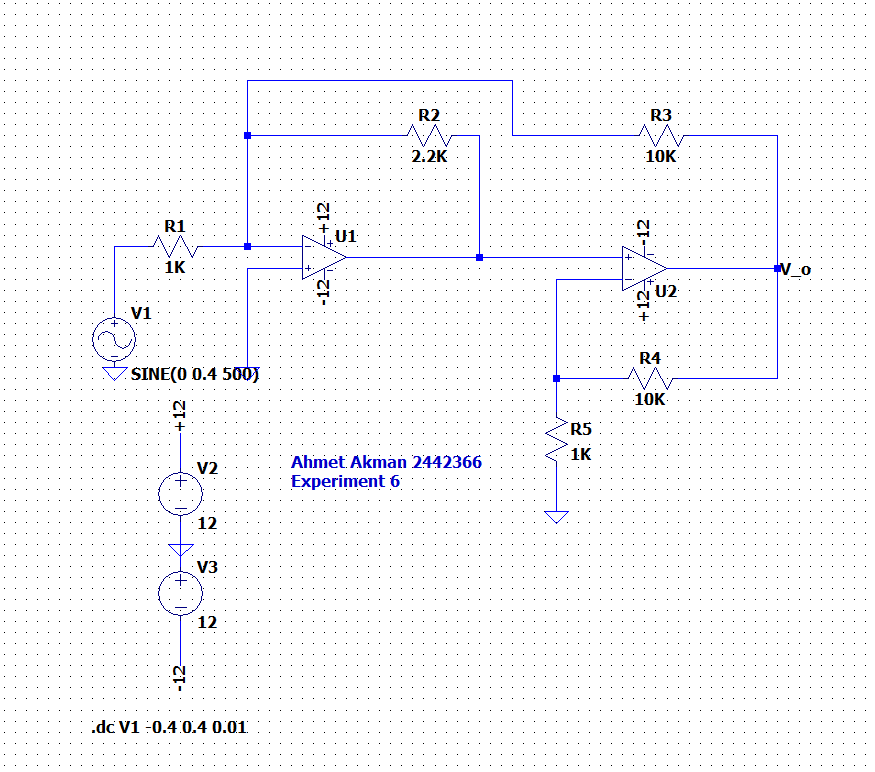
\includegraphics[width=1\textwidth]{Pre1.png}
   \caption{LTSpice schematic for two stage amplifier}
\end{figure} 

Then the plot, \(V_o\) vs \(V_{in}\) is obtained and illustrated in Figure 9.
\begin{figure}[H]
	\centering
   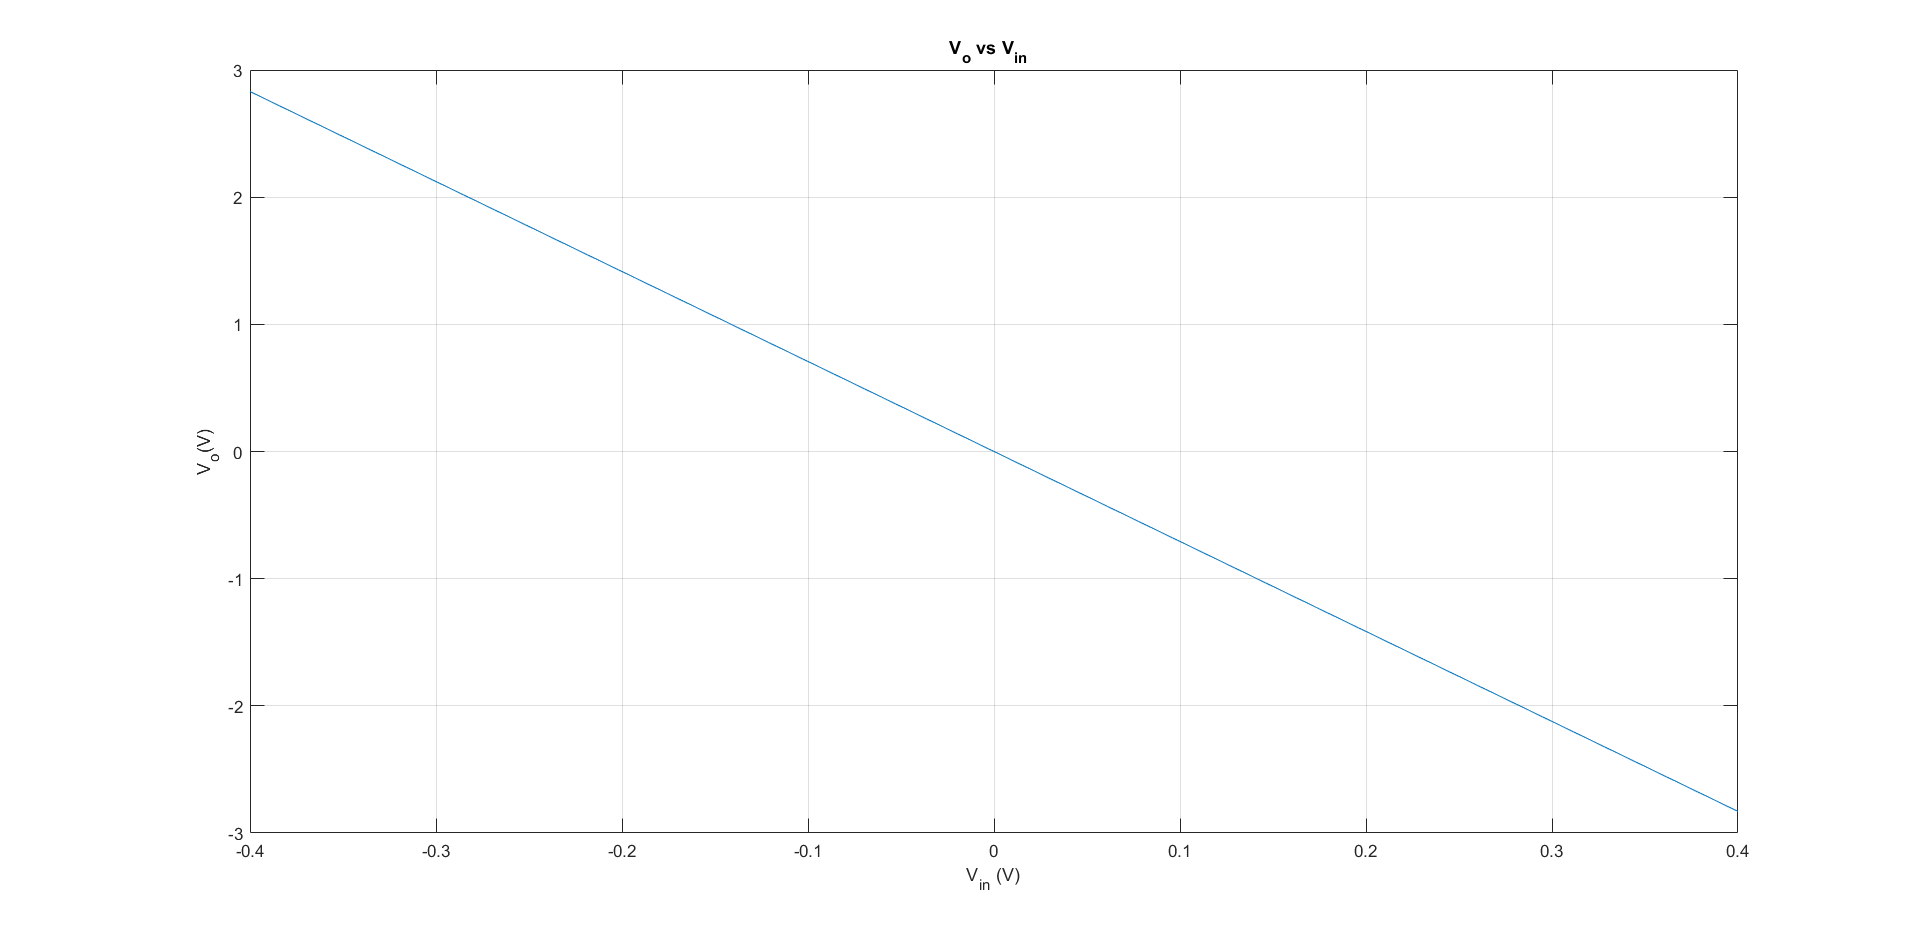
\includegraphics[width=1\textwidth]{Pre_1a.png}
   \caption{\(V_o\) vs \(V_{in}\)}
\end{figure} 
for the part b) of the Step 1 plot given in Figure 10 is obtained.
\begin{figure}[H]
	\centering
   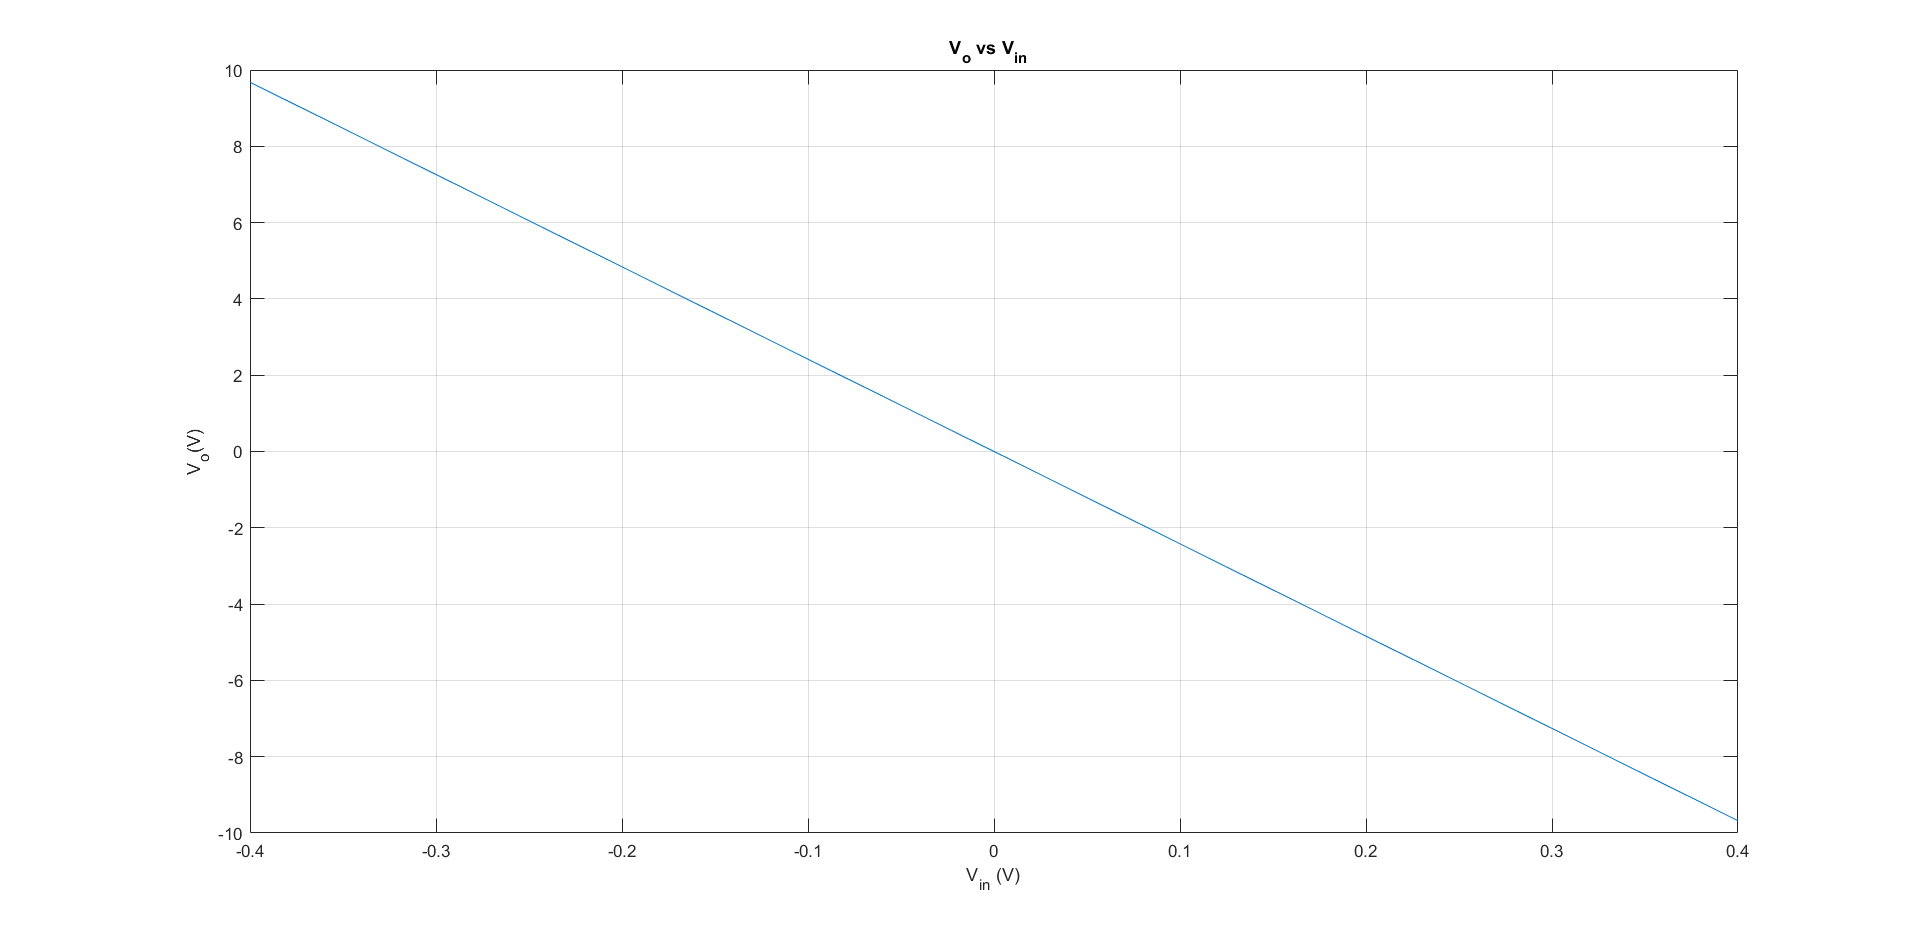
\includegraphics[width=1\textwidth]{Pre_1b.png}
   \caption{\(V_o\) vs \(V_{in}\)}
\end{figure} 
 
By comparing the sketch in the Figure 3, it can be said that simulation result is consistent with our theoretical result.

The circuit in the Figure 5 is constructed in LTSpice environment, given in Figure 12.
\begin{figure}[H]
	\centering
   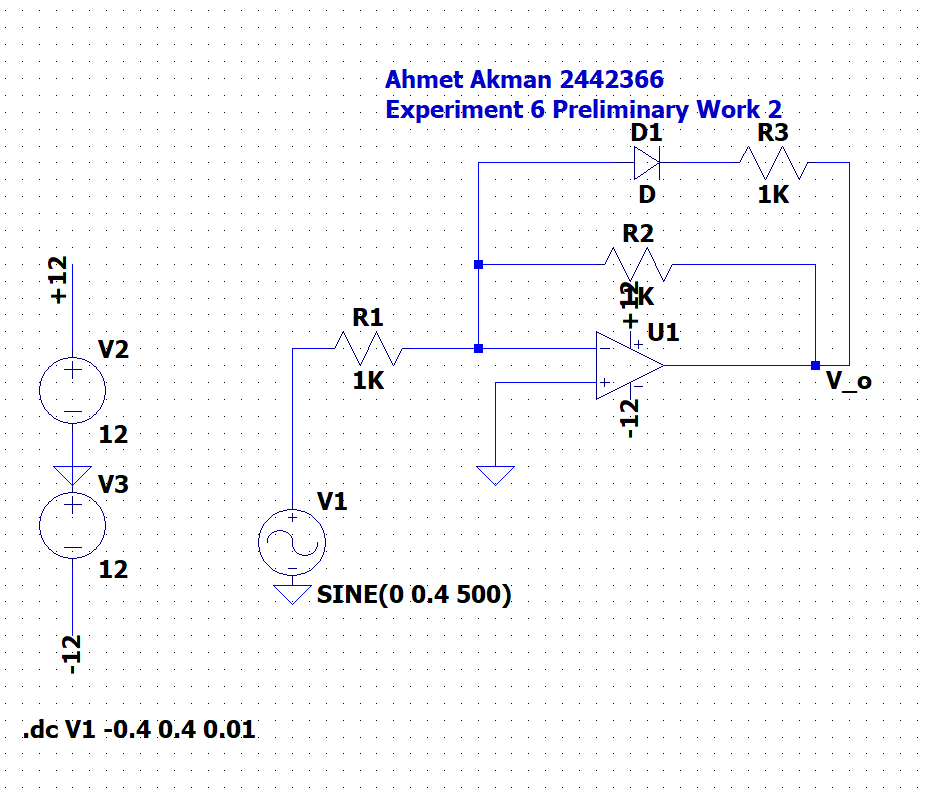
\includegraphics[width=1\textwidth]{Pre2.png}
   \caption{LTSpice schematic for Step 2 circuit}
\end{figure} 


Then the plot, \(V_o\) vs \(V_{in}\) is obtained and illustrated in Figure 13.
\begin{figure}[H]
	\centering
   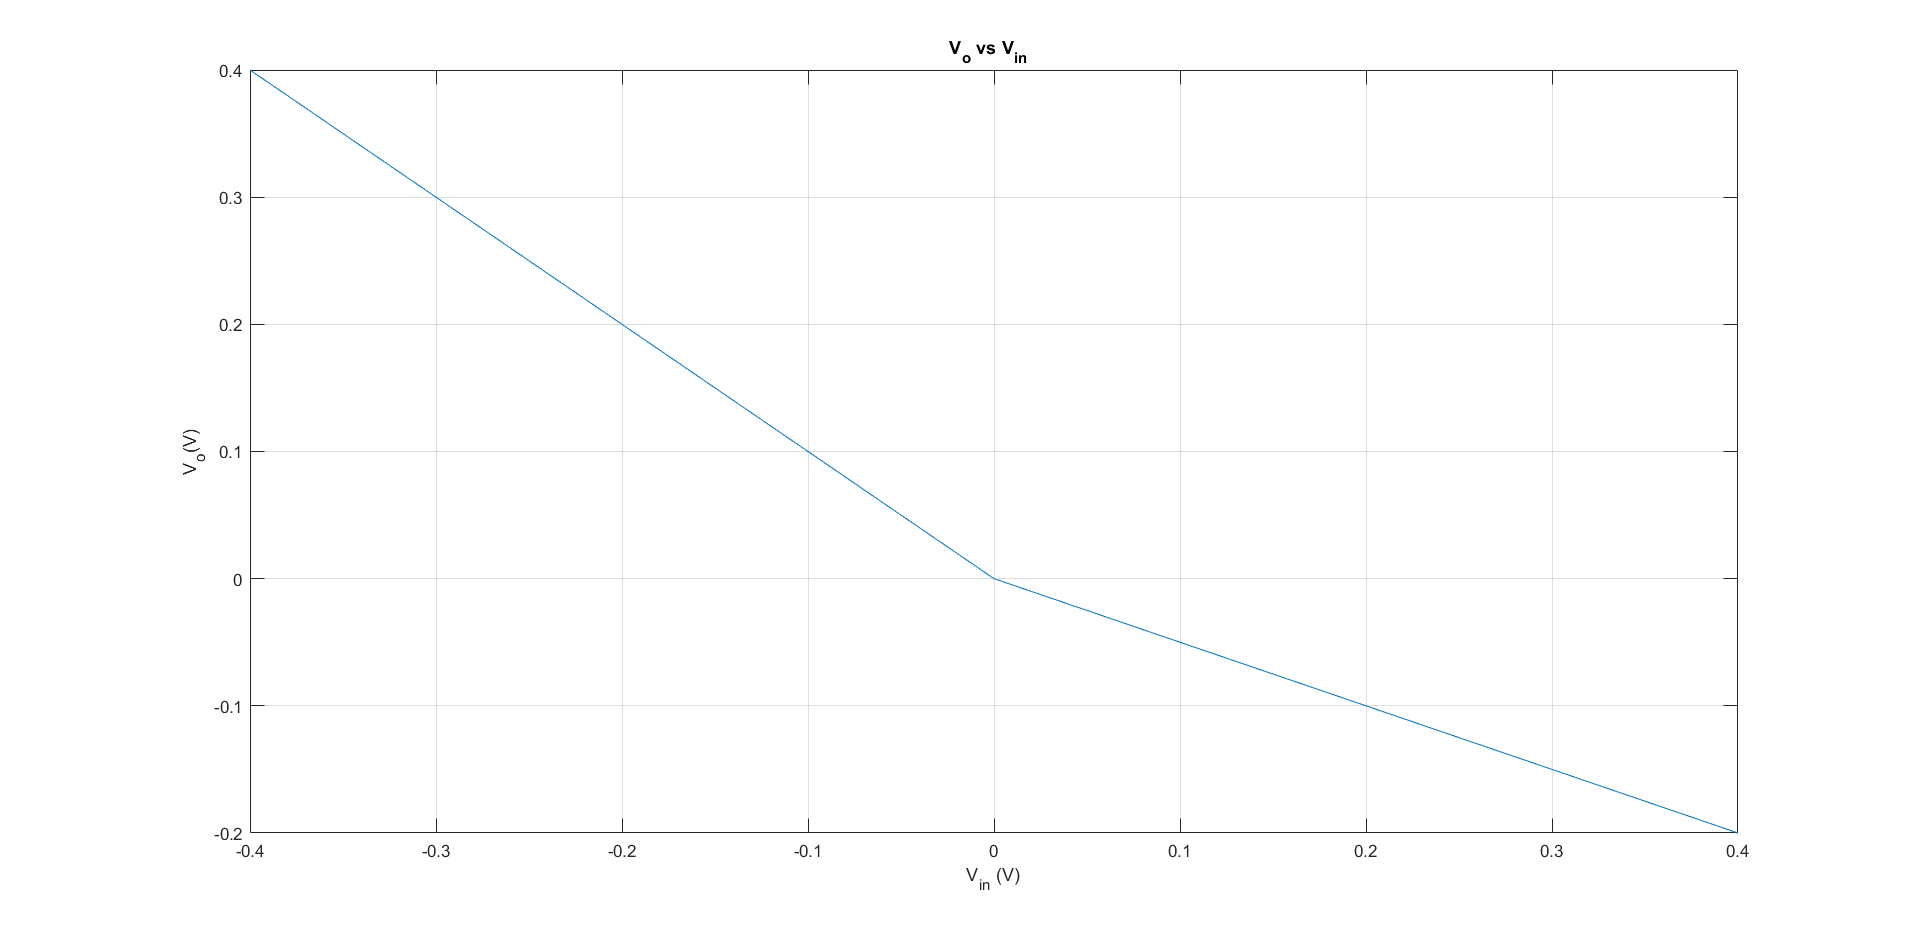
\includegraphics[width=1\textwidth]{Pre_2.png}
   \caption{\(V_o\) vs \(V_{in}\)}
\end{figure} 


By comparing the sketch in the Figure 6, it can be said that simulation result is consistent with our theoretical findings.

\section{Conclusion}
In conclusion, in preliminary work of experiment 6, "Operational Amplifiers-II"  needed the expressions for the amplifier circuits are obtained and necessary data are plotted. Then and simulations are made and compared with theoretical results.

%++++++++++++++++++++++++++++++++++++++++
% References section will be created automatically 
% with inclusion of "thebibliography" environment
% as it shown below. See text starting with line
% \begin{thebibliography}{99}
% Note: with this approach it is YOUR responsibility to put them in order
% of appearance.

%\begin{thebibliography}{99}

%https://tr.overleaf.com/latex/templates/sample-lab-report-for-u-of-r-phys-349/pgsyqngcyjxk

%\end{thebibliography}


\end{document}


\begin{table}[H]
	\begin{center}
		\caption{Resistance reading by color code convention.}
		\vspace{2mm}
		\begin{tabular}{||c | c | c||} 
		 \hline
		 Color Order & Value & Tolerance \\ [0.5ex] 
		 \hline\hline
		 Brown / Black / Red / Gold & 1k\( \Omega \) & \( \% \) 5  \\ 
		 \hline
		 Yellow / Violet / Red / Gold & 4.7k\( \Omega \) & \( \% \) 5   \\
		 \hline
		 Brown / Grey / Orange / Gold & 18k\( \Omega \) & \( \% \) 5  \\ [1ex] 
		 \hline
		\end{tabular}
	\end{center}
	\end{table}

	\begin{figure}[H]
 		\centering
		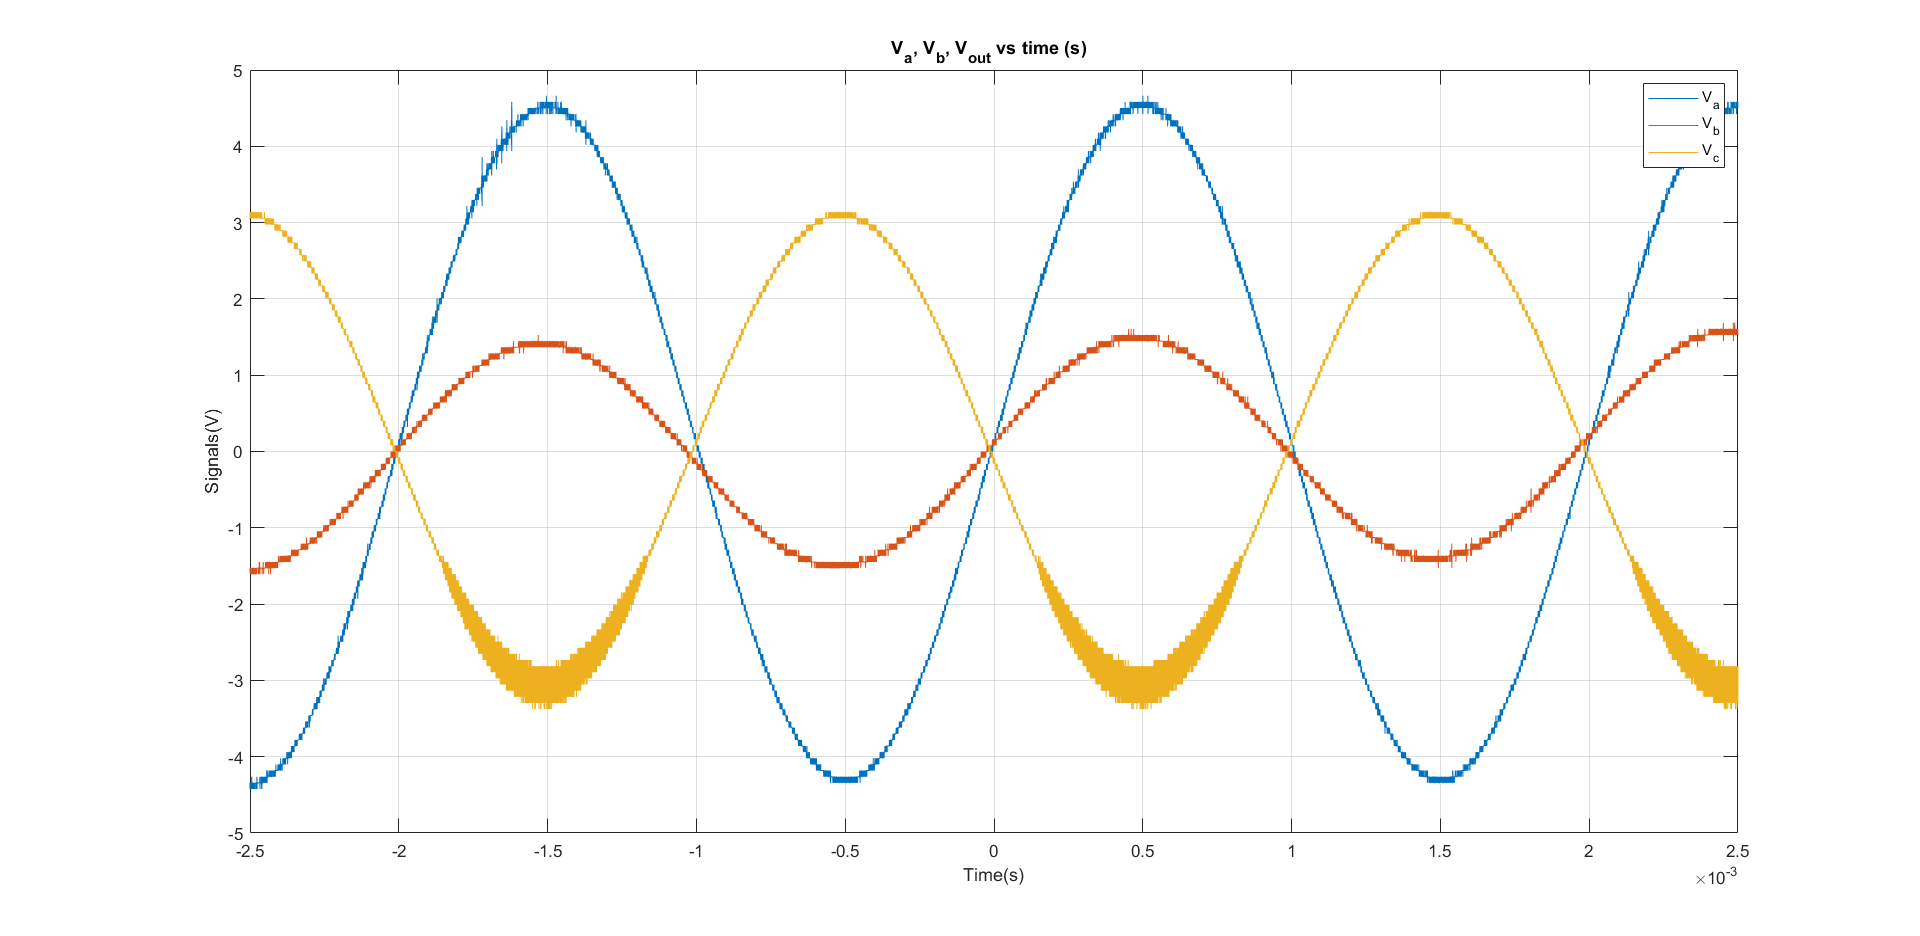
\includegraphics[width=0.6\textwidth]{5.png}
		\caption{Circuit schematic for the step 5}
	\end{figure} 

	\begin{figure}[htp] \centering{
		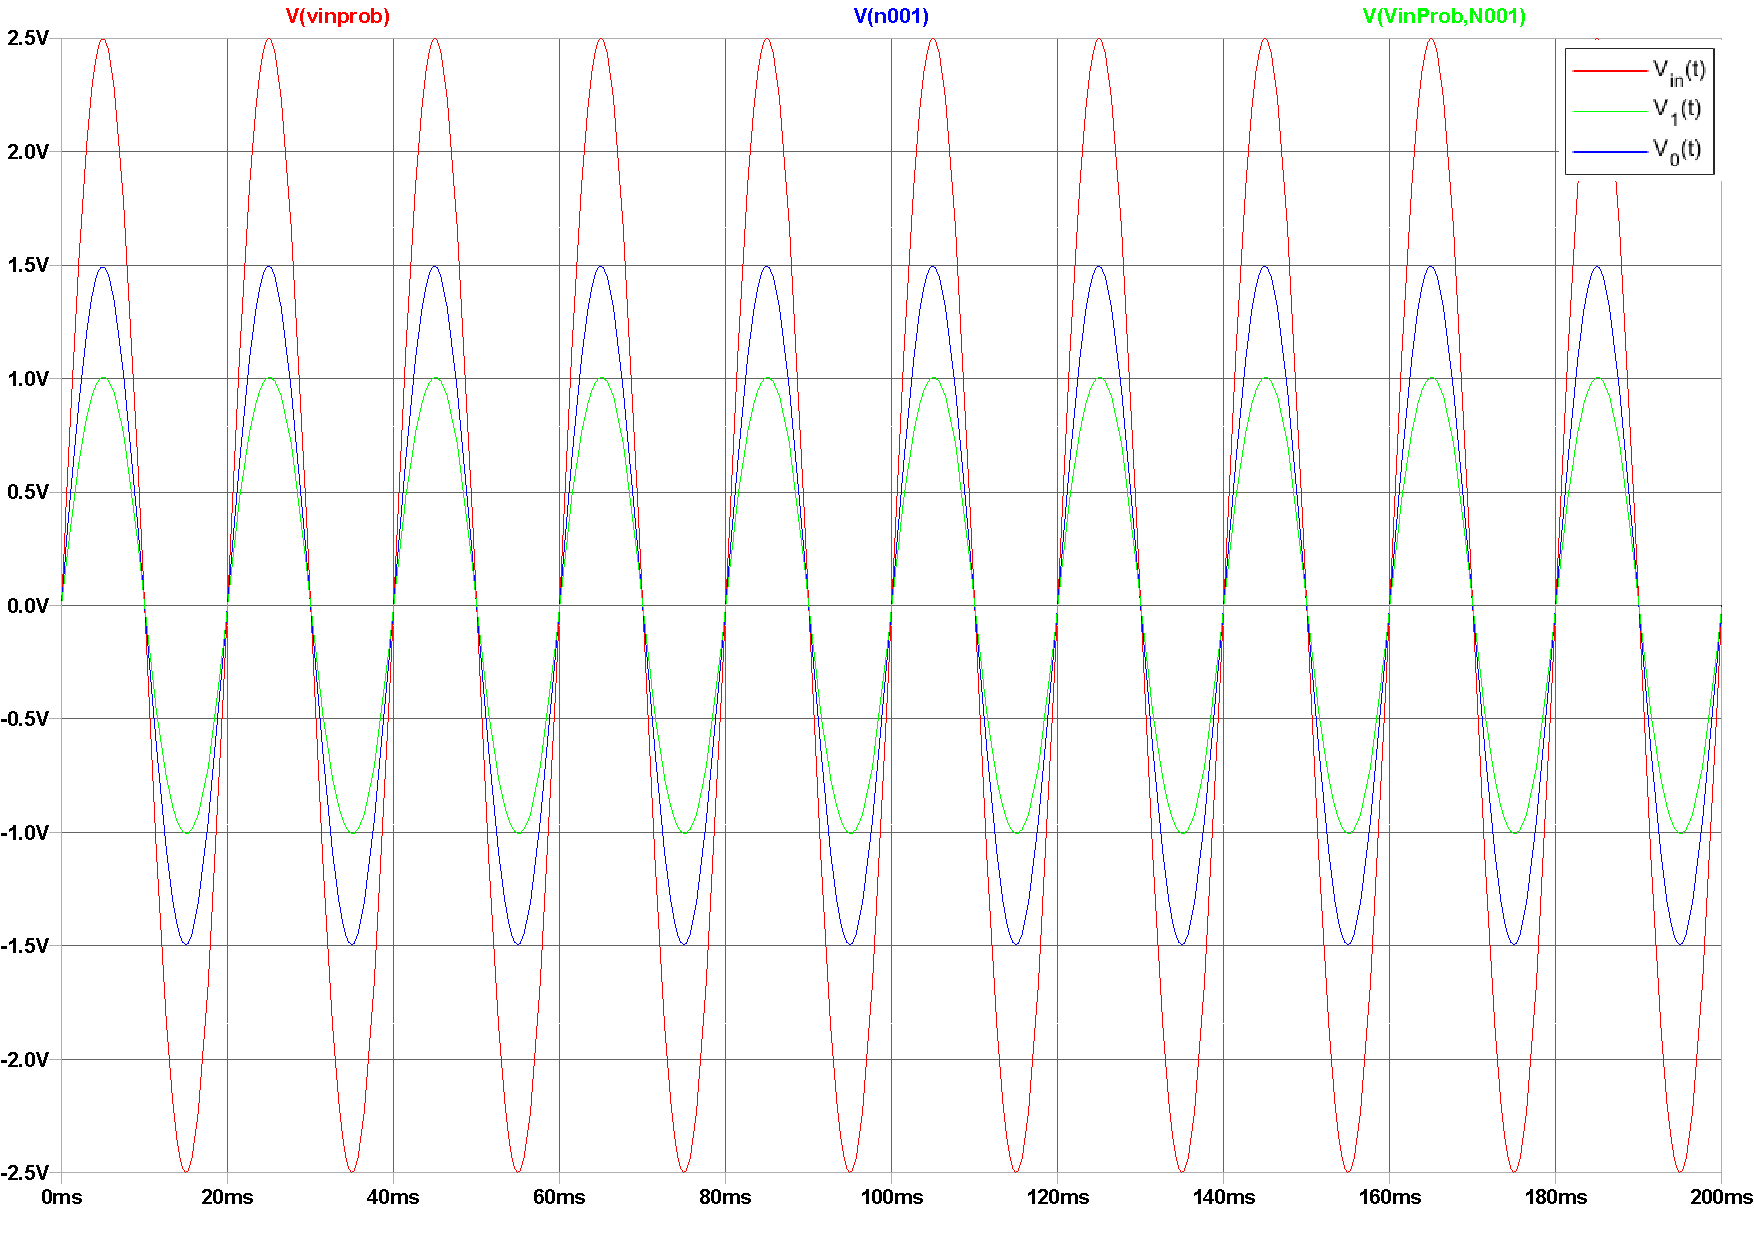
\includegraphics[scale=0.25]{2a_plot.pdf}}
		\caption{Experiment 2}
\end{figure}
	